
%% bare_conf.tex
%% V1.3
%% 2007/01/11
%% by Michael Shell
%% See:
%% http://www.michaelshell.org/
%% for current contact information.
%%
%% This is a skeleton file demonstrating the use of IEEEtran.cls
%% (requires IEEEtran.cls version 1.7 or later) with an IEEE conference paper.
%%
%% Support sites:
%% http://www.michaelshell.org/tex/ieeetran/
%% http://www.ctan.org/tex-archive/macros/latex/contrib/IEEEtran/
%% and
%% http://www.ieee.org/

%%*************************************************************************
%% Legal Notice:
%% This code is offered as-is without any warranty either expressed or
%% implied; without even the implied warranty of MERCHANTABILITY or
%% FITNESS FOR A PARTICULAR PURPOSE! 
%% User assumes all risk.
%% In no event shall IEEE or any contributor to this code be liable for
%% any damages or losses, including, but not limited to, incidental,
%% consequential, or any other damages, resulting from the use or misuse
%% of any information contained here.
%%
%% All comments are the opinions of their respective authors and are not
%% necessarily endorsed by the IEEE.
%%
%% This work is distributed under the LaTeX Project Public License (LPPL)
%% ( http://www.latex-project.org/ ) version 1.3, and may be freely used,
%% distributed and modified. A copy of the LPPL, version 1.3, is included
%% in the base LaTeX documentation of all distributions of LaTeX released
%% 2003/12/01 or later.
%% Retain all contribution notices and credits.
%% ** Modified files should be clearly indicated as such, including  **
%% ** renaming them and changing author support contact information. **
%%
%% File list of work: IEEEtran.cls, IEEEtran_HOWTO.pdf, bare_adv.tex,
%%                    bare_conf.tex, bare_jrnl.tex, bare_jrnl_compsoc.tex
%%*************************************************************************

% *** Authors should verify (and, if needed, correct) their LaTeX system  ***
% *** with the testflow diagnostic prior to trusting their LaTeX platform ***
% *** with production work. IEEE's font choices can trigger bugs that do  ***
% *** not appear when using other class files.                            ***
% The testflow support page is at:
% http://www.michaelshell.org/tex/testflow/



% Note that the a4paper option is mainly intended so that authors in
% countries using A4 can easily print to A4 and see how their papers will
% look in print - the typesetting of the document will not typically be
% affected with changes in paper size (but the bottom and side margins will).
% Use the testflow package mentioned above to verify correct handling of
% both paper sizes by the user's LaTeX system.
%
% Also note that the "draftcls" or "draftclsnofoot", not "draft", option
% should be used if it is desired that the figures are to be displayed in
% draft mode.
%
\documentclass[conference]{IEEEtran}
% Add the compsoc option for Computer Society conferences.
%
% If IEEEtran.cls has not been installed into the LaTeX system files,
% manually specify the path to it like:
% \documentclass[conference]{../sty/IEEEtran}

\usepackage{pdfsync}
\usepackage{comment}
\usepackage{amsmath}
\usepackage{amssymb}
\usepackage{amsthm}
\usepackage{calc}
\usepackage{color}
\usepackage{graphicx}
\usepackage{url}
\usepackage{xspace}
\usepackage{tikz}
\usepackage{pgfplots}
\usepackage{caption}
\usepackage{subcaption}
\usepackage{xspace}
\usepackage{color}
\usepackage{booktabs}


\usepackage[algo2e, noend, noline, linesnumbered]{algorithm2e}
\DontPrintSemicolon

\makeatletter
\newcommand{\pushline}{\Indp}% Indent
\newcommand{\popline}{\Indm}
\makeatother
\DeclareMathOperator{\pess}{pess}
\DeclareMathOperator{\opti}{opti}
\newcommand{\argmax}{\operatornamewithlimits{argmax}}
\newcommand{\defword}[1]{\textbf{\boldmath{#1}}}

\captionsetup{compatibility=false}

%\pgfplotsset{compat=newest}
\usetikzlibrary{arrows,shapes,petri}

\newcommand{\bE}{\mathbb{E}}
\newcommand{\bQ}{\bar{Q}}
\newcommand{\cA}{\mathcal{A}}
\newcommand{\cC}{\mathcal{C}}
\newcommand{\cD}{\mathcal{D}}
\newcommand{\cG}{\mathcal{G}}
\newcommand{\cI}{\mathcal{I}}
\newcommand{\cN}{\mathcal{N}}
\newcommand{\cO}{\mathcal{O}}
\newcommand{\cR}{\mathcal{R}}
\newcommand{\cS}{\mathcal{S}}
\newcommand{\cT}{\mathcal{T}}
\newcommand{\cZ}{\mathcal{Z}}
\newcommand{\hQ}{\hat{Q}}
\newcommand{\hV}{\hat{V}}
\newcommand{\eg}{{\it e.g.,}~}
\newcommand{\ie}{{\it i.e.,}~}
\newtheorem{definition}{Definition}
\newtheorem{fact}{Fact}
\newtheorem{theorem}{Theorem}
\newtheorem{corollary}{Corollary}
\newtheorem{lemma}{Lemma}
\newtheorem{proposition}{Proposition}
\newcommand{\Proof}{{\noindent\bf Proof. }}
\newcommand{\citejustyear}[1]{\cite{#1}}
\newcommand{\Qed}{$\blacksquare$}
\newcommand{\abs}[1]{\left|#1\right|}
\newcommand{\todo}[1]{{\color{red}{\bf #1}}}
\newcommand{\breturn}{{\bf return}\xspace}

% the note center!
\definecolor{darkgreen}{RGB}{0,125,0}
\newcounter{nsNoteCounter}
\newcounter{mlNoteCounter}
\newcounter{mwNoteCounter}
\newcounter{tpNoteCounter}
\newcommand{\nsnote}[1]{{\scriptsize \color{blue} $\blacksquare$ \refstepcounter{vlNoteCounter}\textsf{[NS]$_{\arabic{vlNoteCounter}}$:{#1}}}}
\newcommand{\mlnote}[1]{{\scriptsize \color{darkgreen} $\blacksquare$ \refstepcounter{mlNoteCounter}\textsf{[ML]$_{\arabic{mlNoteCounter}}$:{#1}}}}
\newcommand{\mwnote}[1]{{\scriptsize \color{red} $\blacktriangle$ \refstepcounter{asNoteCounter}\textsf{[AS]$_{\arabic{asNoteCounter}}$:{#1}}}}
\newcommand{\tpnote}[1]{{\scriptsize \color{orange} $\blacktriangle$ \refstepcounter{asNoteCounter}\textsf{[TP]$_{\arabic{asNoteCounter}}$:{#1}}}}
%\newcounter{NoteCounter}
%\newcommand{\vlnote}[1]{{\scriptsize \color{blue} \refstepcounter{vlNoteCounter}\textsf{[VL]$_{\arabic{vlNoteCounter}}$:{#1}}}}
%\renewcommand{\vlnote}[1]{}



% Some very useful LaTeX packages include:
% (uncomment the ones you want to load)


% *** MISC UTILITY PACKAGES ***
%
%\usepackage{ifpdf}
% Heiko Oberdiek's ifpdf.sty is very useful if you need conditional
% compilation based on whether the output is pdf or dvi.
% usage:
% \ifpdf
%   % pdf code
% \else
%   % dvi code
% \fi
% The latest version of ifpdf.sty can be obtained from:
% http://www.ctan.org/tex-archive/macros/latex/contrib/oberdiek/
% Also, note that IEEEtran.cls V1.7 and later provides a builtin
% \ifCLASSINFOpdf conditional that works the same way.
% When switching from latex to pdflatex and vice-versa, the compiler may
% have to be run twice to clear warning/error messages.






% *** CITATION PACKAGES ***
%
%\usepackage{cite}
% cite.sty was written by Donald Arseneau
% V1.6 and later of IEEEtran pre-defines the format of the cite.sty package
% \cite{} output to follow that of IEEE. Loading the cite package will
% result in citation numbers being automatically sorted and properly
% "compressed/ranged". e.g., [1], [9], [2], [7], [5], [6] without using
% cite.sty will become [1], [2], [5]--[7], [9] using cite.sty. cite.sty's
% \cite will automatically add leading space, if needed. Use cite.sty's
% noadjust option (cite.sty V3.8 and later) if you want to turn this off.
% cite.sty is already installed on most LaTeX systems. Be sure and use
% version 4.0 (2003-05-27) and later if using hyperref.sty. cite.sty does
% not currently provide for hyperlinked citations.
% The latest version can be obtained at:
% http://www.ctan.org/tex-archive/macros/latex/contrib/cite/
% The documentation is contained in the cite.sty file itself.






% *** GRAPHICS RELATED PACKAGES ***
%
\ifCLASSINFOpdf
  % \usepackage[pdftex]{graphicx}
  % declare the path(s) where your graphic files are
  % \graphicspath{{../pdf/}{../jpeg/}}
  % and their extensions so you won't have to specify these with
  % every instance of \includegraphics
  % \DeclareGraphicsExtensions{.pdf,.jpeg,.png}
\else
  % or other class option (dvipsone, dvipdf, if not using dvips). graphicx
  % will default to the driver specified in the system graphics.cfg if no
  % driver is specified.
  % \usepackage[dvips]{graphicx}
  % declare the path(s) where your graphic files are
  % \graphicspath{{../eps/}}
  % and their extensions so you won't have to specify these with
  % every instance of \includegraphics
  % \DeclareGraphicsExtensions{.eps}
\fi
% graphicx was written by David Carlisle and Sebastian Rahtz. It is
% required if you want graphics, photos, etc. graphicx.sty is already
% installed on most LaTeX systems. The latest version and documentation can
% be obtained at: 
% http://www.ctan.org/tex-archive/macros/latex/required/graphics/
% Another good source of documentation is "Using Imported Graphics in
% LaTeX2e" by Keith Reckdahl which can be found as epslatex.ps or
% epslatex.pdf at: http://www.ctan.org/tex-archive/info/
%
% latex, and pdflatex in dvi mode, support graphics in encapsulated
% postscript (.eps) format. pdflatex in pdf mode supports graphics
% in .pdf, .jpeg, .png and .mps (metapost) formats. Users should ensure
% that all non-photo figures use a vector format (.eps, .pdf, .mps) and
% not a bitmapped formats (.jpeg, .png). IEEE frowns on bitmapped formats
% which can result in "jaggedy"/blurry rendering of lines and letters as
% well as large increases in file sizes.
%
% You can find documentation about the pdfTeX application at:
% http://www.tug.org/applications/pdftex





% *** MATH PACKAGES ***
%
%\usepackage[cmex10]{amsmath}
% A popular package from the American Mathematical Society that provides
% many useful and powerful commands for dealing with mathematics. If using
% it, be sure to load this package with the cmex10 option to ensure that
% only type 1 fonts will utilized at all point sizes. Without this option,
% it is possible that some math symbols, particularly those within
% footnotes, will be rendered in bitmap form which will result in a
% document that can not be IEEE Xplore compliant!
%
% Also, note that the amsmath package sets \interdisplaylinepenalty to 10000
% thus preventing page breaks from occurring within multiline equations. Use:
%\interdisplaylinepenalty=2500
% after loading amsmath to restore such page breaks as IEEEtran.cls normally
% does. amsmath.sty is already installed on most LaTeX systems. The latest
% version and documentation can be obtained at:
% http://www.ctan.org/tex-archive/macros/latex/required/amslatex/math/





% *** SPECIALIZED LIST PACKAGES ***
%
%\usepackage{algorithmic}
% algorithmic.sty was written by Peter Williams and Rogerio Brito.
% This package provides an algorithmic environment fo describing algorithms.
% You can use the algorithmic environment in-text or within a figure
% environment to provide for a floating algorithm. Do NOT use the algorithm
% floating environment provided by algorithm.sty (by the same authors) or
% algorithm2e.sty (by Christophe Fiorio) as IEEE does not use dedicated
% algorithm float types and packages that provide these will not provide
% correct IEEE style captions. The latest version and documentation of
% algorithmic.sty can be obtained at:
% http://www.ctan.org/tex-archive/macros/latex/contrib/algorithms/
% There is also a support site at:
% http://algorithms.berlios.de/index.html
% Also of interest may be the (relatively newer and more customizable)
% algorithmicx.sty package by Szasz Janos:
% http://www.ctan.org/tex-archive/macros/latex/contrib/algorithmicx/




% *** ALIGNMENT PACKAGES ***
%
%\usepackage{array}
% Frank Mittelbach's and David Carlisle's array.sty patches and improves
% the standard LaTeX2e array and tabular environments to provide better
% appearance and additional user controls. As the default LaTeX2e table
% generation code is lacking to the point of almost being broken with
% respect to the quality of the end results, all users are strongly
% advised to use an enhanced (at the very least that provided by array.sty)
% set of table tools. array.sty is already installed on most systems. The
% latest version and documentation can be obtained at:
% http://www.ctan.org/tex-archive/macros/latex/required/tools/


%\usepackage{mdwmath}
%\usepackage{mdwtab}
% Also highly recommended is Mark Wooding's extremely powerful MDW tools,
% especially mdwmath.sty and mdwtab.sty which are used to format equations
% and tables, respectively. The MDWtools set is already installed on most
% LaTeX systems. The lastest version and documentation is available at:
% http://www.ctan.org/tex-archive/macros/latex/contrib/mdwtools/


% IEEEtran contains the IEEEeqnarray family of commands that can be used to
% generate multiline equations as well as matrices, tables, etc., of high
% quality.


%\usepackage{eqparbox}
% Also of notable interest is Scott Pakin's eqparbox package for creating
% (automatically sized) equal width boxes - aka "natural width parboxes".
% Available at:
% http://www.ctan.org/tex-archive/macros/latex/contrib/eqparbox/





% *** SUBFIGURE PACKAGES ***
%\usepackage[tight,footnotesize]{subfigure}
% subfigure.sty was written by Steven Douglas Cochran. This package makes it
% easy to put subfigures in your figures. e.g., "Figure 1a and 1b". For IEEE
% work, it is a good idea to load it with the tight package option to reduce
% the amount of white space around the subfigures. subfigure.sty is already
% installed on most LaTeX systems. The latest version and documentation can
% be obtained at:
% http://www.ctan.org/tex-archive/obsolete/macros/latex/contrib/subfigure/
% subfigure.sty has been superceeded by subfig.sty.



%\usepackage[caption=false]{caption}
%\usepackage[font=footnotesize]{subfig}
% subfig.sty, also written by Steven Douglas Cochran, is the modern
% replacement for subfigure.sty. However, subfig.sty requires and
% automatically loads Axel Sommerfeldt's caption.sty which will override
% IEEEtran.cls handling of captions and this will result in nonIEEE style
% figure/table captions. To prevent this problem, be sure and preload
% caption.sty with its "caption=false" package option. This is will preserve
% IEEEtran.cls handing of captions. Version 1.3 (2005/06/28) and later 
% (recommended due to many improvements over 1.2) of subfig.sty supports
% the caption=false option directly:
%\usepackage[caption=false,font=footnotesize]{subfig}
%
% The latest version and documentation can be obtained at:
% http://www.ctan.org/tex-archive/macros/latex/contrib/subfig/
% The latest version and documentation of caption.sty can be obtained at:
% http://www.ctan.org/tex-archive/macros/latex/contrib/caption/




% *** FLOAT PACKAGES ***
%
%\usepackage{fixltx2e}
% fixltx2e, the successor to the earlier fix2col.sty, was written by
% Frank Mittelbach and David Carlisle. This package corrects a few problems
% in the LaTeX2e kernel, the most notable of which is that in current
% LaTeX2e releases, the ordering of single and double column floats is not
% guaranteed to be preserved. Thus, an unpatched LaTeX2e can allow a
% single column figure to be placed prior to an earlier double column
% figure. The latest version and documentation can be found at:
% http://www.ctan.org/tex-archive/macros/latex/base/



%\usepackage{stfloats}
% stfloats.sty was written by Sigitas Tolusis. This package gives LaTeX2e
% the ability to do double column floats at the bottom of the page as well
% as the top. (e.g., "\begin{figure*}[!b]" is not normally possible in
% LaTeX2e). It also provides a command:
%\fnbelowfloat
% to enable the placement of footnotes below bottom floats (the standard
% LaTeX2e kernel puts them above bottom floats). This is an invasive package
% which rewrites many portions of the LaTeX2e float routines. It may not work
% with other packages that modify the LaTeX2e float routines. The latest
% version and documentation can be obtained at:
% http://www.ctan.org/tex-archive/macros/latex/contrib/sttools/
% Documentation is contained in the stfloats.sty comments as well as in the
% presfull.pdf file. Do not use the stfloats baselinefloat ability as IEEE
% does not allow \baselineskip to stretch. Authors submitting work to the
% IEEE should note that IEEE rarely uses double column equations and
% that authors should try to avoid such use. Do not be tempted to use the
% cuted.sty or midfloat.sty packages (also by Sigitas Tolusis) as IEEE does
% not format its papers in such ways.





% *** PDF, URL AND HYPERLINK PACKAGES ***
%
%\usepackage{url}
% url.sty was written by Donald Arseneau. It provides better support for
% handling and breaking URLs. url.sty is already installed on most LaTeX
% systems. The latest version can be obtained at:
% http://www.ctan.org/tex-archive/macros/latex/contrib/misc/
% Read the url.sty source comments for usage information. Basically,
% \url{my_url_here}.





% *** Do not adjust lengths that control margins, column widths, etc. ***
% *** Do not use packages that alter fonts (such as pslatex).         ***
% There should be no need to do such things with IEEEtran.cls V1.6 and later.
% (Unless specifically asked to do so by the journal or conference you plan
% to submit to, of course. )


% correct bad hyphenation here
%\hyphenation{op-tical net-works semi-conduc-tor}


\begin{document}
%
% paper title
% can use linebreaks \\ within to get better formatting as desired
\title{Monte Carlo Tree Search with Heuristic Evaluations\\using Implicit Minimax Backups}


% author names and affiliations
% use a multiple column layout for up to three different
% affiliations

%\author{Author1 Author2 Author3 Author4}

\author{\IEEEauthorblockN{Marc Lanctot$^1$, Tom Pepels$^1$, Mark H.~M. Winands$^1$, and Nathan R. Sturtevant$^2$}
\IEEEauthorblockA{$^1$Department of Knowledge Engineering, Maastricht University}
\IEEEauthorblockA{$^2$Computer Science Department, University of Denver}
\{marc.lanctot,tom.pepels,m.winands\}@maastrichtuniversity.nl, sturtevant@cs.du.edu}
%\IEEEauthorblockA{Twentieth Century Fox\\
%Springfield, USA\\
%Email: homer@thesimpsons.com}
%\and
%\IEEEauthorblockN{James Kirk\\ and Montgomery Scott}
%\IEEEauthorblockA{Starfleet Academy\\
%San Francisco, California 96678-2391\\
%Telephone: (800) 555--1212\\
%Fax: (888) 555--1212}}

% conference papers do not typically use \thanks and this command
% is locked out in conference mode. If really needed, such as for
% the acknowledgment of grants, issue a \IEEEoverridecommandlockouts
% after \documentclass

% for over three affiliations, or if they all won't fit within the width
% of the page, use this alternative format:
% 
%\author{\IEEEauthorblockN{Michael Shell\IEEEauthorrefmark{1},
%Homer Simpson\IEEEauthorrefmark{2},
%James Kirk\IEEEauthorrefmark{3}, 
%Montgomery Scott\IEEEauthorrefmark{3} and
%Eldon Tyrell\IEEEauthorrefmark{4}}
%\IEEEauthorblockA{\IEEEauthorrefmark{1}School of Electrical and Computer Engineering\\
%Georgia Institute of Technology,
%Atlanta, Georgia 30332--0250\\ Email: see http://www.michaelshell.org/contact.html}
%\IEEEauthorblockA{\IEEEauthorrefmark{2}Twentieth Century Fox, Springfield, USA\\
%Email: homer@thesimpsons.com}
%\IEEEauthorblockA{\IEEEauthorrefmark{3}Starfleet Academy, San Francisco, California 96678-2391\\
%Telephone: (800) 555--1212, Fax: (888) 555--1212}
%\IEEEauthorblockA{\IEEEauthorrefmark{4}Tyrell Inc., 123 Replicant Street, Los Angeles, California 90210--4321}}




% use for special paper notices
%\IEEEspecialpapernotice{(Invited Paper)}




% make the title area
\maketitle


\begin{abstract}
Monte Carlo Tree Search (MCTS) has improved the performance of game-playing engines in 
domains such as Go, Hex, and general-game playing. MCTS has been shown to outperform
outperform classic alpha-beta search in games where good heuristic evaluations are difficult to obtain. 
In recent years, combining ideas from traditional minimax search in MCTS has been shown to be advantageous in some domains, 
such as Lines of Action, Amazons, and Breakthrough.
In this paper, we propose 
a new way to use heuristic evaluations to guide the MCTS search by storing the two sources of 
information, estimated win rates and heuristic evaluations, separately. 
Rather than using the heuristic evaluations to replace the playouts, 
our technique backs them up {\it implicitly} during its MCTS simulations. 
These learned evaluation values are then used to guide future simulations. 
Compared to current techniques, we show that using implicit minimax backups  
leads to stronger play performance in Breakthrough, Lines of Action, and Kalah. 
\end{abstract}
% IEEEtran.cls defaults to using nonbold math in the Abstract.
% This preserves the distinction between vectors and scalars. However,
% if the conference you are submitting to favors bold math in the abstract,
% then you can use LaTeX's standard command \boldmath at the very start
% of the abstract to achieve this. Many IEEE journals/conferences frown on
% math in the abstract anyway.

% no keywords




% For peer review papers, you can put extra information on the cover
% page as needed:
% \ifCLASSOPTIONpeerreview
% \begin{center} \bfseries EDICS Category: 3-BBND \end{center}
% \fi
%
% For peerreview papers, this IEEEtran command inserts a page break and
% creates the second title. It will be ignored for other modes.
\IEEEpeerreviewmaketitle

%%% paper content
\section{Introduction}

Monte Carlo Tree Search (MCTS)~\cite{Coulom06Efficient,Kocsis06Bandit} is a simulation-based best-first
search paradigm that has been shown to increase performance in domains such as turn-taking games, 
general-game playing, real-time strategy games, single-agent planning, and more~\cite{mctssurvey}. 
While the initial applications have been to games where heuristic evaluations are difficult to obtain, 
progress in MCTS research has shown that heuristics can be effectively be combined in MCTS, even in games 
where classic minimax search has traditionally been preferred. 

The most popular MCTS algorithm is UCT~\cite{Kocsis06Bandit}, 
which performs a single simulation from the root of the search tree to a terminal state at each iteration. 
During the iterative process, a game tree is incrementally built by adding a 
new leaf node to the tree on each iteration, whose nodes track statistical estimates such average payoffs. 
With each new simulation, these estimates improve and help to guide future simulations. 

%The nodes in the tree are used to store statistical information regarding wins and losses, and backpropagation
%policies are used to update parent estimates, and these improving estimates are then used to select actions 
%during simulations. 
%When the simulation reaches parts of the game tree not included in the model, a default playout policy
%is used to simulate to a terminal state where a win or loss is determined. 

%When applied to sequential turn-taking games, MCTS has primarily been used in domains where good 
%heuristic evaluations are difficult to obtain. 
In this work, we propose a new technique to augment the quality of MCTS simulations with  
an implicitly-computed minimax search which uses heuristic evaluations. 
Unlike previous work, these heuristic evaluations are used as {\it separate source of information}, 
and backed up in the same way as in classic minimax search. Furthermore, these minimax-style 
backups are done {\it implicitly},
as a simple extra step during the standard updates to the tree nodes, and always maintained 
separately from win rate estimates obtained from playouts. These two separate information 
sources are then used to guide MCTS simulations. 
We show that combining heuristic evaluations in this way can lead to significantly stronger play performance in three 
separate domains: Breakthrough, Kalah, and Lines of Action. 

\subsection{Related Work}

Several techniques for minimax-influenced backup rules in the simulation-based MCTS framework have been previously proposed. 
The first was Coulom's original {\it maximum backpropagation}~\cite{Coulom06Efficient}. This method of backpropagation
suggests, after a number of simulations to a node has been reached, to switch to propagating the maximum value instead 
of the simulated (average) value. 
The rationale behind this choice is that after a certain point, the search algorithm should consider a node
{\it converged} and return an estimate of the best value. 
Maximum backpropagation has also recently been used in other Monte Carlo tree search algorithms and demonstrated success in
probabilistic planning, as an alternative type of forecaster in BRUE~\cite{Feldman13Theoretically} and as Bellman 
backups for online dynamic programming in Trial-based Heuristic Tree Search~\cite{Keller13Trial}.

The first use of enhancing MCTS using prior knowledge was in Computer Go~\cite{Gelly07Combining}. 
In this work, offline-learned knowledge initialized values of expanded nodes increased performance against significantly against 
strong benchmark player. 
This technique was also confirmed to be advantageous in Breakthrough~\cite{Lorentz13Breakthrough}. 
Another way to introduce prior knowledge is via a progressive bias during selection~\cite{Chaslot08Progressive}, which has 
significantly increased performance in Go play strength~\cite{Chaslot10Adding}. 

In games where minimax search performs well, such as Kalah, 
modifying MCTS to use minimax-style backups and heuristic values instead to replace playouts offers a worthwhile trade-off 
under different search time settings~\cite{Ramanujan11Tradeoffs}.
Similarly, there is further evidence suggesting not replacing the playout entirely, but terminating them early 
using heuristic evaluations, has increased the performance in Lines of Action (LOA)~\cite{Winands10MCTS-LOA}, 
Amazons~\cite{Kloetzer10Amazons,Lorentz08Amazons}, and Breakthrough~\cite{Lorentz13Breakthrough}. In LOA and Amazons, the 
MCTS players enhanced with evaluation functions outperform their minimax counterparts using the same evaluation function.

% mention score-bounded mcts
% mention hendrik's minimax methods
% use mcts-solver to motivate implicit minimax
%\marcl{Also mention MCTS + minimax hybrids (Baier \& Winands) and Score-bounded MCTS (...))}


One may want to combine minimax backups or searches without using an evaluation function. 
The prime example is MCTS-Solver~\cite{Winands08Solver}, which backpropagates proven wins and losses as 
extra information in MCTS. When a node is proven to be a 
win or a loss, it no longer needs to be searched. This domain-independent modification greatly enhances 
MCTS with negligible overhead. Score-bounded MCTS extends this idea to games with multiple 
outcomes, leading to $\alpha \beta$-style pruning in the tree~\cite{Cazenave10Score}. Finally, one can use hybrid
minimax searches in the tree to initialize nodes during, enhance the playout, or to help MCTS-Solver 
in backpropagation~\cite{Baier13MinimaxHybrids}.

Finally, recent work has attempted to explain and identify some of the shortcomings that arise from estimates in 
MCTS, specifically compared to situations where classic minimax search has historically performed 
well~\cite{Ramanujan10Understanding,Ramanujan10On}. 
Attempts have been made to overcome the problem of {\it traps} or {\it optimistic moves}, \ie moves that initially seem 
promising but then later prove to be bad, such as sufficiency 
thresholds~\cite{Gudmindsson13Sufficiency} and shallow minimax searches~\cite{Baier13MinimaxHybrids}. 

%We show that implicit minimax backups also improve performance in domains with tactical short-term goals. 

\section{Adversarial Search in Turn-Taking Games}

%The following notation is taken from~\cite{Sutton98}

A finite deterministic Markov Decision Process (MDP) is 4-tuple $(\cS, \cA, \cT, \cR)$. Here, $\cS$ is a finite non-empty set of {\it states}. 
$\cA$ is a finite non-empty set of {\it actions}, where we denote $\cA(s) \subseteq \cA$ the set of available actions at state $s$. 
$\cT : \cS \times \cA \mapsto \Delta \cS$ is a {\it transition function} mapping 
each state and action to a distribution over successor states. Finally, $\cR : \cS \times \cA \times \cS \mapsto R$ 
is a {\it reward function} mapping (state, action, successor state) triplets to numerical rewards. 

A two-player perfect information game is an MDP with a specific form. 
Denote $\cZ = \{ s \in \cS: \cA(s) = \emptyset \} \subset \cS$ the set of {\it terminal states}. 
In addition, for all nonterminal states $s' \in \cS - \cZ$, $\cR(s,a,s') = 0$. 
There is a {\it player identity function} $\tau : \cS - \cZ \mapsto \{1,2\}$. 
The rewards $\cR(s,a,s')$ are always with respect to the same player and  
we assume zero-sum games so that rewards with respect to the opponent player are simply negated. 
In this paper, we assume fully deterministic domains, so $\cT(s,a)$ maps $s$ to a single successor 
state. 
However, the ideas proposed can be easily extended to domains with stochastic transitions. 
When it is clear from the context and unless otherwise stated, we denote $s' = \cT(s,a)$. 

Monte Carlo Tree Search is a simulation-based best-first search algorithm that incrementally builds a tree, $\cG$, 
in memory. 
Each search starts with from a {\it root state} $s_0 \in \cS - \cZ$, and initially sets $\cG = \emptyset$. 
Each simulation samples a trajectory $\rho = (s_0, a_0, s_1, a_1, \cdots, s_n)$, where $s_n \in \cZ$ unless the playout 
is terminated early. 
The portion of the $\rho$ where $s_i \in \cG$ is called the {\it tree portion} and the remaining portion is
called the {\it playout portion}. In the tree portion, actions are chosen according to some {\it selection policy}. 
The first state encountered in the playout portion is {\it expanded}, added to $\cG$.
The actions chosen in the playout portion are determined by a specific {\it playout policy}. 
States $s \in \cG$ are referred to as {\it nodes} and statistics are  
maintained for each node $s$: the cumulative reward, $r_s$, and visit count, $n_s$. 
By popular convention, we define $r_{s,a} = r_{s'}$ where $s' = \cT(s,a)$, and similarly $n_{s,a} = n_{s'}$. 
Also, we use $r^{\tau}_s$ to denote the reward at state $s$ {\it with respect to player} $\tau(s)$. 
%Finally, we denote  the set $C(s)$ to be the children of $s$ that are in $\cG$. 

Let $\hV(s)$ an estimator of the win rate starting from node $s$ and $\hQ(s,a)$ for the state-action pair. 
For example, one popular estimator is the observed mean over all simulations 
$\bQ(s,a) = r^{\tau}_{s,a} / n_{s,a}$. 
The most widely-used selection policy is based on a bandit algorithm called Upper Confidence Bounds 
(UCB)~\cite{Auer02Finite}, used in adaptive multistage sampling~\cite{Chang2005AMS} and in 
UCT~\cite{Kocsis06Bandit}, which selects action $a'$ using
\begin{equation}
\label{eq:select-ucb}
a' = \argmax_{a \in \cA(s)} \left\{ \hQ(s,a) + C \sqrt{\frac{\ln n_s}{n_{s,a}}} \right\}, 
\end{equation}
where $C$ is parameter determining the weight of exploration. 

\section{Implicit Minimax Backups in MCTS}

Our proposed technique is based on the following principle: if an evaluation function is available, then it should 
be possible for MCTS to make use of it, and it should at least never {\it hurt} performance. 
But, how could MCTS use this information to account for short-term strategic goals, such as maximizing piece scores?

Suppose we are given an evaluation function $v_0(s)$ whose range is the same as that of the reward function $\cR$. 
How should MCTS make use of this information? 
Assuming $v_0(s)$ is a sensible indicator of the reward, we would like that this added source of information
strictly benefits MCTS. 
We propose a simple and elegant solution: add another value to maintain at each node, the 
{\it implicit minimax evaluation with respect to player} $\tau(s)$, $v^{\tau}_s$, with $v^{\tau}_{s,a}$ defined similarly 
as above. 
This new value at node $s$ {\it only} maintains a heuristic minimax value built from the evaluations of subtrees below $s$. 
During backpropagation, $r_s$ and $n_s$ are updated in the usual way, and additionally $v^{\tau}_s$ is updated using minimax backup 
rule based on children values. Then, similarly to RAVE~\cite{Gelly07Combining}, rather than using $\hQ = \bQ$ for 
selection in Equation~\ref{eq:select-ucb}, we use
\begin{equation}
\label{eq:imq}
\hQ^{\mathit{IM}}(s,a) = (1-\alpha) \frac{r^{\tau}_{s,a}}{n_{s,a}} + \alpha v^{\tau}_{s,a}, 
\end{equation}
where $\alpha$ is a weight representing the influence of the heuristic minimax values.

The entire process is summarized in Algorithm~\ref{alg}. There are three simple additions to vanilla MCTS,
%which are located on lines \ref{alg:imselect}, \ref{alg:imeval}, and \ref{alg:imexpand}.
which are located on lines 2, 8, and 13.
During selection, $\hQ^{\mathit{IM}}$ from Equation~\ref{eq:imq} replaces $\bQ$ in 
Equation~\ref{eq:select-ucb}. During backpropagation, the implicit minimax evaluations $v^{\tau}_s$ are updated based on 
the children's values. For simplicity, a single $\max$ operator is used here since the evaluations are assumed to be in 
view of player $\tau(s)$. Depending on how the game is modeled, the implementation may require keeping track of or  
accounting for signs of rewards. For example a negamax model would include a sign switches at the appropriate places 
to ensure that the payoffs are in view of the current player at each node.  
%line~\ref{alg:imeval}. 
%\footnote{Domain-dependent inversions or scalings may be necessary to convert the rewards. These details are 
%intentionally omitted from the pseudo-code for generality.}
%The function $\alpha(n_s)$ will determine how much weight to attribute to these evaluations.  
Finally, after a node expansion, on 13, the implicit minimax value is initialized to its heuristic
evaluation $v^{\tau}_s \leftarrow v^{\tau}_0(s)$. 

\newcommand{\MCTS}{{\sc MCTS}}
\newcommand{\Update}{{\sc Update}}
\newcommand{\Playout}{{\sc Playout}}
\newcommand{\Select}{{\sc Select}}
\newcommand{\Expand}{{\sc Expand}}
\newcommand{\Simulate}{{\sc Simulate}}

\begin{algorithm2e}[t!]
  \Select$(s)$:\;
  \pushline
    Let $A'$ be the set of actions $a \in \cA(s)$ maximizing $\hQ^{\mathit{IM}}(s,a) + C \sqrt{\frac{\ln n_s}{n_{s,a}}}$ \; 
    {\bf return} $a' \sim ${\sc Uniform}$(A')$ \;
  \popline
  \;
  \Update$(s,r)$:\;
  \pushline
    $r_s \leftarrow r_s + r$\;
    $n_s \leftarrow n_s + 1$\;
    $v^{\tau}_s \leftarrow \max_{a \in \cA(s)} v^{\tau}_{s,a}$ \; 
  \popline
  \;
  \Simulate$(s_{prev}, a_{prev}, s)$:\;
  \pushline
    \If{$s \not\in \cG$}{
      \Expand($s$)\;        
      $v^{\tau}_s \leftarrow v^{\tau}_0(s)$ \; 
      $r \leftarrow $\Playout($s$)\;
      \Update($s,r$)\;
      {\bf return} $r$\;                       
    }
    \Else{ 
      \lIf{$s \in \cZ$}{{\bf return} $\cR(s_{prev}, a_{prev}, s)$}
      $a \leftarrow $\Select$(s)$\;
      $s' \leftarrow \cT(s,a)$\;
      $r \leftarrow $\Simulate$(s,a,s')$\;
      \Update($s,r$)\;
      {\bf return} $r$\;                      
    }
  \popline
  \;
  \MCTS($s_0$):\;
  \pushline
    \lWhile{\mbox{time left}}{\Simulate$(-,-,s_0)$}
    {\bf return} $\argmax_{a \in \cA(s_0)} n_{s_0,a}$\; 
  \popline
  \vspace{0.3cm}
  \caption{MCTS with implicit minimax backups. \label{alg}}
\end{algorithm2e}

In essence, MCTS with implicit minimax backups acts like a heuristic approximation of MCTS-Solver for the portion of the
search tree that has not reached terminal states. 
However, unlike MCTS-Solver and minimax hybrids, these modifications are based on heuristic evaluations rather than 
proven wins and losses.
%which might help the search in the opening and mid-games. 

%While a badly chosen-evaluation function can still converge to the optimal value eventually with a minimax-consistent
%backup rule, we are mainly concerned with how an evaluation function can help MCTS performance.
%Our empirical evaluation will show that MCTS can benefit significantly from this added information, even with 
%simple heuristic evaluation functions.

\section{Empirical Evaluation}

\newcommand{\UCTMAXH}{$\mbox{UCTMAX}_H$\xspace}
\newcommand{\UCTH}{$\mbox{UCT}_H$\xspace}

In this section, we thoroughly evaluate the practical performance of the implicit minimax backups technique. 
Before reporting head-to-head results, we first describe our experimental setup and 
summarize the techniques that have been used to improve playouts. We then present results on three game
domains: Breakthrough, Kalah, and Lines of Action. 

Unless otherwise stated, our implementations expand a new node every simulation, the first node encountered
that is not in the tree. MCTS-Solver is enabled in all of our experiments since its overhead is negligible and
never decreases performance. After the simulations are done, the final move chosen is the one with the highest
number of visits. 
Rewards are in $\{-1, 0, 1\}$ representing a loss, draw, and win.
To ensure values in the same range, evaluation functions are scaled to $[-1,1]$ by passing a domain-dependent 
score differences through a cache-optimized sigmoid function. 
When simulating, to avoid memory overhead, a single game state is modified and 
moves are undone when returning from the recursive call.
Whenever possible, evaluation functions are updated incrementally to save time. 
All of the experiments include swapped seats to ensure that each player type plays 
an equal number of games as first player and as second player.
All reported win rates are over 1000 played games unless specifically stated otherwise, such as in Lines of Action.
Domain-dependent playout policies and optimizations are reported in each subsection.

We compare to and combine our technique with number of previous ones to include  
domain knowledge. A popular recent technique is {\it early playout terminations}. When a leaf node of the tree 
is reached, a fixed-depth early playout terminations, hereby abbreviated to ``fet$x$'', plays $x$ moves according
to the playout policy resulting in state $s$, and then terminates the playout returning $v_0(s)$. This method has
shown to improve performance against standard MCTS in Amazons, Kalah, and 
Breakthrough~\cite{Lorentz08Amazons,Ramanujan11Tradeoffs,Lorentz13Breakthrough}. 

A similar technique is {\it dynamic early terminations}, which periodically checks the evaluation function 
(or other domain-dependent features) terminating only when some condition is met. 
This approach has been used as a ``mercy rule'' in Go~\cite{Bouzy07Old} and quite successfully in 
Lines of Action~\cite{Winands08MCTSSolver}.
In our version, which we abbreviate ``det$x$'', a playout is terminated and returns $1$ if $v_0(s) \ge x$ and 
$-1$ if $v_0(s) \le -x$. Another option is to use an $\epsilon$-greedy playout policy that chooses a successor randomly 
with probability $\epsilon$ and successor state with the largest evaluation with probability $1-\epsilon$, with 
improved performance in Chinese Checkers~\cite{Sturtevant08An,Nijssen12Playout}, abbreviated ``ege$\epsilon$''.

To facilitate the discussion, 
we will refer to each enhancement and setting using different labels. These enhancements and labels are described in 
the text that follows. But, we also include, for reference, a summary of each in Table~\ref{table:enhancements}.

To tune parameters in Kalah and Breakthrough, we ran hierarchical elimination tournaments against players of 
the same type where each head-to-head match consisted of 200 games with seats swapped halfway. 
All of the detailed results of these tournaments comparisons are contained in Appendix A.\footnote{Appendix A is supplementary material, located 
at \url{http://mlanctot.info/tmp/mctsim-app.pdf}. If the paper is accepted, the details in this appendix 
will be made available as part of a follow-up technical report.}

\begin{table}[tb]
{\small
\caption{Enhancements tested in Kalah (K), Breakthrough (B), and Lines of Action (L).}
\begin{center}
\begin{tabular}{|l|c|c|c|c|}
\hline 
Enhancement / Setting       & Abbr.          & K           & B           & L \\ 
\hline                                                                   
Early playout termination   & fet$x$         & \checkmark  & \checkmark  &            \\
Dynamic early termination   & det$x$         &             & \checkmark  & \checkmark \\
$\epsilon$-greedy playouts  & ege$\epsilon$  &             & \checkmark  &            \\
Node priors                 & np             &             & \checkmark  &            \\
Maximum backpropagation     &                &             & \checkmark  &            \\
Progressive bias            & PB             &             & \checkmark  & \checkmark \\
$\alpha\beta$ playouts      &                &             &             & \checkmark \\
\hline                                                                   
Implicit minimax backups    & im$\alpha$     & \checkmark  & \checkmark  & \checkmark \\
\hline                                                                   
Simple evaluation function  & efRS, efMS     & \checkmark  & \checkmark  &            \\
Sophisticated ev. function  & efLH, efWB     &             & \checkmark  & \checkmark \\
Baseline player              & bl            &             & \checkmark  &            \\
Alternative baseline settings & bl'          &             & \checkmark  &            \\
\hline
\end{tabular}
\end{center} 
\label{table:enhancements} }
\end{table}%

\subsection{Kalah}

\begin{figure}
\begin{center}
\includegraphics[scale=0.68]{plots/kalah-alpha}
\caption{Results in Kalah. Each data point is based on roughly 1000 games; win percentages are $\pm \approx$ 3.0\% 
with 95\% confidence.}
\label{fig:kalah-alpha}
\end{center}
\end{figure}

Kalah is a turn-taking game in the Mancala family of games. Each player has six houses, each 
initially containing four stones, and a store on the endpoint of the board, initially empty. 
On their turn, a player chooses one of their houses, removes all the stones in it, and ``sows'' 
the stones one per house in counter-clockwise fashion, skipping the opponent's store. 
If the final stone lands in the player's store, that player gets another turn, and there is no 
limit to then number of consecutive turns taken by same player. If the stone ends on a house owned
by the player that contains no stones, then that player captures all the stones in the adjacent 
opponent house, putting it into the player's store. The game plays until one player's houses are
all empty; the opponent then moves their remaining stones to their store. The winner is the player
who has collected the most stones in their store. 
Kalah has been weakly solved for several different variants of Kalah~\cite{Irving00Solving}, 
and was used as a domain to compare MCTS variants to classic minimax search~\cite{Ramanujan11Tradeoffs}.

In running experiments from the initial position, we observed a noticeable first-player bias. Therefore, as
was done in \cite{Ramanujan11Tradeoffs}, our experiments produce random starting board positions 
without any stones placed in the stores. 
Competing players play one game and then swap seats to play a second game using the same board. A player 
is declared a winner if that player won one of the games and at least tied the other game. If the same side 
wins both games, the game is discarded. 

We then determined which playout enhancement led to the best baseline player. 
Tournament results revealed that a fet$4$ early termination worked best. 

The evaluation function was the same one used in \cite{Ramanujan11Tradeoffs}, the difference between stones
in each player's stores. Results with one 
second of search time are shown in Figure~\ref{fig:kalah-alpha}. 
%As with the previous study employing MCTS, we notice that an evaluation function can be used to enhance the performance.
%Here, we again notice the same patterns as in Breakthrough. 
Here, we notice that within the range $\alpha \in [0.1,0.5]$ there is a clear 
advantage in performance when using implicit minimax backups against the base player. 
This graph has a recurring shape that we have seen in our other domains as well. 

\subsection{Breakthrough}
\label{sec:bt}

Breakthrough is a turn-taking alternating move game played on an 8-by-8 chess board. Each player 
has 16 identical pieces on their first two rows. 
A piece is allowed to move forward to an empty square, either straight or diagonal, but may only 
capture diagonally like Chess pawns. A player wins by moving a single piece to the furthest opponent row. 

Breakthrough was first introduced in general game-playing competitions and has been identified as a domain 
that is particularly difficult for MCTS due to traps and uninformed playouts~\cite{Gudmindsson13Sufficiency}. 
Our playout policy always chooses a one-ply ``decisive'' wins and prevents immediate ``anti-decisive'' 
losses~\cite{Teytaud10On}.
Otherwise, a move is selected non-uniformly at random, where capturing undefended pieces are four times more
likely than other moves. 
MCTS with this informed playout policy beats the one using uniform random 94.3\% of the time. Therefore, this 
playout policy leads to a clear improvement over random playouts, and so we so we only use it for the rest 
of our experiments. 

We use two evaluation functions. The first one is a simple one found in Maarten Schadd's thesis~\cite{Schadd11PhdThesis} 
that assigns each piece a score of 10 and the further row achieved as 2.5, which we abbreviate ``efMS''. The second 
one is the more sophisticated one giving specific point values for each individual square per player 
described in a recent paper by Lorentz \& Horey~\cite{Lorentz13Breakthrough}, which we abbreviate ``efLH''. 
We base much of our analysis in Breakthrough on the Lorentz \& Horey player, which 
at the time of publication had an ELO rating of 1910 on the Little Golem web site. 
Currently, the ELO rating is 2098 which is the 4th highest out of over 300 Breakthrough players. 


%Another popular technique is {\it maximimum backpropagation}, where certain number of visits in the \Update~procedure,
%the valued backed up is the one of the best child instead of the sampled value from the simulation.
%Couloum originally showed that the the mean backpropagation to be superior in Go~\cite{Coulom06Efficient}. 
%In Kalah, the \UCTMAXH algorithm proposed by Ramanujan resembles closely maximum backpropagation with early terminations 
%(pd0) except that the values are also weighted by visit counts, and was shown to perform as well or better than a strong minimax 
%player at a low number of nodes expansions. Another successful technique in Go is 
%{\it node priors}~\cite{Gelly07Combining}, where newly-expanded nodes are assigned some initial wins and loss counts, 
%which also improved performance in Breakthrough~\cite{Lorentz13Breakthrough}. Finally, another way to use 
%heuristic knowledge is as a means of {\it progressive bias} which has been rather successful
%in Go~\cite{Gelly07Combining,ChaslotWHUB2008} and Lines of Action~\cite{Winands10MCTS-LOA}.

\begin{figure}[t]
\begin{center}
\includegraphics[scale=0.7]{plots/bt-base-alpha}\\
\includegraphics[scale=0.7]{plots/bt-basenp-alpha}
\caption{Results in Breakthrough against 
baseline player MCTS(ege$0.1$,det$0.5$). The implicit minimax player uses efMS. 
Each point represents 1000 games. The top graph excludes node priors, bottom graph includes node priors.} 
\label{fig:bt-base-alpha}
\end{center}
\end{figure}

Our first set of experiments uses the simple evaluation function, efMS. At the end of this subsection, we 
include experiments for the sophisticated evaluation function efLH.

We first determined the best playout strategy amongst fixed and dynamic early 
terminations and $\epsilon$-greedy playouts.
Our best fixed early terminations player was fet$20$ and best $\epsilon$-greedy player was ege$0.1$.
Through systematic testing on 1000 games per pairing, we determined that the best playout 
policy when using efMS is the combination (ege$0.1$,det$0.5$), which 
we call the baseline player, abbreviated as ``bl''. The detailed test results are found in Appendix A.
To ensure that this combination of early termination strategies is indeed superior to just the informed 
playout policy on its own, we also played it against MCTS using just informed playout policy on its own, 
and MCTS(ege$0.1$,det$0.5$) won 68.8\% of these games.
MCTS(ege$0.1$,det$0.5$) is the best baseline
player that we could produce given three separate parameter-tuning tournaments, for all the playout enhancements 
we have tried using efMS, over thousands of played games. Hence, we 
use it as our primary benchmark for comparison in the the rest of our experiments, (ege$0.1$,det$0.5$) is 
used as the playout policy for every MCTS player unless otherwise stated.
As a final summary, this baseline player:
\begin{enumerate}
\item Uses ege$0.1$, an $\epsilon$-greedy playout policy with $\epsilon = 0.1$.
\item Uses det$0.5$, dynamic early terminations where a playout is terminated early if the evaluation 
      of the state surpasses the thresholds of $<-0.5$ and $>+0.5$.
\end{enumerate}

%however is likely explained by less 
%overhead due to incremental evaluations and efficient transitions. 

We then played MCTS with implicit minimax backups, MCTS(im$\alpha$), against this baseline player for a 
variety different values for $\alpha$. The results are shown in the top of Figure~\ref{fig:bt-base-alpha}.
Implicit minimax backups give an advantage for $\alpha \in [0.1,0.6]$ under both one- and five-second 
search times. 
When $\alpha > 0.6$, MCTS(im$\alpha$) acts like greedy best-first minimax.
To verify that the benefit was not only due to the optimized playout policy, we performed two experiments. 
First, we played MCTS(im$0.4$) against an MCTS player where both players were forced to to use playout policy 
without any early terminations (but still informed as mentioned above), and MCTS(im$0.4$) won 82.3\% of these games. 
We then played MCTS(im$0.4$) against an MCTS player where both players used fet$20$, and
MCTS(fet$20$,im$0.4$) won 87.2\% of these games.

%\begin{figure}[t]
%\begin{center}
%\newgame
%\def\mylist{Pa1, Pb1, Pc1, Pd1, Pe1, Pf1, Ph1, Pg1, pd6, pe7}
%\setchessboard{setpieces=\mylist,showmover=false}
%\chessboard
%\end{center}
%\caption{An example position in Breakthrough. \mlnote{I hope to have a nice example to show here soon.}}
%\end{figure}
 
The next question was whether the mixing static evaluation values themselves ($v_0(s)$) at node $s$ 
was the source of the benefit or whether the minimax backup values ($v^{\tau}_s$) were the contributing factor.
Therefore, we tried MCTS(bl, im$0.4$) against a baseline player that uses constant bias over the static 
evaluations, \ie uses an estimator
\[ \hQ^{CB}(s,a) = (1-\alpha)\bQ + \alpha v_0(s'),\] 
in line 2, and also against a player using a progressive bias over the minimax backups, \ie 
\[ \hQ^{PB}(s,a) = (1-\alpha)\bQ + \alpha v^{\tau}_s/(n_{s,a} + 1)\]
in line 2.
MCTS(bl,im$0.4$) won 67.8\% against MCTS(bl,$\hQ^{CB}$). 
MCTS(bl,im$0.4$) won 65.5\% against MCTS(bl,$\hQ^{PB}$). 
It is possible that a different decay function for $v^{\tau}_s$ will further improve the advantage, and we leave 
this as an interesting topic for future work. 

Another question is whether to prefer implicit minimax backups over {\it node priors} (np)~\cite{Gelly07Combining}, 
\ie initializing each new leaf node with wins and losses based on prior knowledge. This technique showed initial
success in Go, but has also been applied with success to path planning problems~\cite{Eyerich10High}.
In our case, we use the node priors that worked well in~\cite{Lorentz13Breakthrough}
which takes into account the safety of surrounding pieces, and scaled the counts by the 
time setting (10 for one second, 50 for five seconds).
We ran MCTS(im$\alpha$) against the baseline player where both players use node priors. 
The results are shown at the bottom of Figure~\ref{fig:bt-base-alpha}. When combined at one second of 
search time, implicit minimax backups still seem to give an advantage for $\alpha \in [0.5,0.6]$, and at five 
seconds gives an advantage for $\alpha \in [0.1,0.6]$. To verify that the combination is complementary,
we played MCTS(im$0.6$) with and without node priors each against the baseline player. The player with
node priors won 77.9\% and, from Figure 1, the one without won 63.3\%. 

We then evaluated MCTS(im$0.4$) against {\it maximum backpropagation} proposed as an alternative 
backpropagation in the original MCTS work~\cite{Coulom06Efficient}. This enhancement
%modifies line \ref{alg:retline2} of the algorithm to the following: 
modifies line 23 of the algorithm to the following: 
\[
\mathbf{if}~n_{s} \ge T~\mathbf{then~return}~\max_{a \in \cA(s)} \bQ(s,a)~\mathbf{else~return}~r.
\]
The results for several values of $T$ are given in Table~\ref{tbl:maxbackprop}. 

\begin{table}[t]
{\small
\begin{center}
\begin{tabular}{|c|ccccccc|}
\hline
                     & \multicolumn{7}{|c|}{$T$ (in thousands)}             \\
Time                & 0.1  & 0.5  & 1    & 5    & 10   & 20 & 30 \\
\hline
1s                 & 81.9 & 73.1 & 69.1 & 65.2 & 63.6 & 66.2 & 67.0 \\
%5s                  &      &      &      &      &      &      &      \\  
\hline
\end{tabular}
\end{center}
\caption{Win rates (\%) of MCTS(im$0.4$) vs. maximum backpropagation in Breakthrough, 
for $T \in \{ 100, \cdots, 30000 \}$. }
\label{tbl:maxbackprop}
}
\end{table}

%            mcts_h_ege0.1_efv0_det0.5 vs.      mcts_h_pd20_np10:   402   598     0 (diff  -196, games  1000) 40.20 59.80 +/- 3.04
%            mcts_h_ege0.1_efv0_det0.5 vs.       mcts_h_pd4_np10:   576   424     0 (diff   152, games  1000) 57.60 42.40 +/- 3.06
% mcts_h_ege0.1_efv0_det0.5_np10_im0.6 vs.      mcts_h_pd20_np10:   849   151     0 (diff   698, games  1000) 84.90 15.10 +/- 2.22
% mcts_h_ege0.1_efv0_det0.5_np10_im0.6 vs.       mcts_h_pd4_np10:   886   114     0 (diff   772, games  1000) 88.60 11.40 +/- 1.97
%       mcts_h_ege0.1_efv0_det0.5_np10 vs.      mcts_h_pd20_np10:   780   220     0 (diff   560, games  1000) 78.00 22.00 +/- 2.57
%       mcts_h_ege0.1_efv0_det0.5_np10 vs.       mcts_h_pd4_np10:   692   308     0 (diff   384, games  1000) 69.20 30.80 +/- 2.86
%       mcts_h_ege0.1_efv0_det0.5_im0.4 vs.	   mcts_h_ege0.1_efv0_det0.5_mbp20000:   662   338     0 (diff   324, games  1000) 66.20 33.80 +/- 2.93
%       mcts_h_ege0.1_efv0_det0.5_im0.4 vs.	   mcts_h_ege0.1_efv0_det0.5_mbp50000:   670   330     0 (diff   340, games  1000) 67.00 33.00 +/- 2.91

\subsubsection*{MCTS Using Lorentz \& Horey Evaluation Function}

We now run experiments using the more sophisticated evaluation function from~\cite{Lorentz13Breakthrough}, 
efLH, that assigns specific piece count values depending on their position on the board. 
Rather than repeating all of the above experiments, we chose simply to compare baselines and to repeat
the initial experiment, all using 1 second of search time.

The best playout with this evaluation function is fet$20$ with node priors, which we call the alternative baseline, 
abbreviated `` bl' ''.
We reran the initial $\alpha$ experiment using the alternative baseline, 
which uses the Lorentz \& Horey evaluation function, to find the best implicit minimax player using this 
more sophisticated evaluation function. Results are shown in Figure~\ref{fig:bt-alt-alpha}. 
In this case the best range is $\alpha \in [0.5,0.6]$ for one second and $\alpha \in [0.5,0.6]$ for
five seconds.
We label the best player in this figure using the alternative baseline MCTS(efLH,bl',im$0.6$). 

In an effort to explain the relative strengths of each evaluation function, we then compared the two baseline players. 
Our baseline MCTS player, MCTS(efMS,bl), wins 40.2\% of games against the alternative baseline, MCTS(efLH,bl'). 
When we add node priors, MCTS(efMS,bl,np) wins 78.0\% of games against MCTS(efLH,bl'). 
When we also add implicit minimax backups ($\alpha = 0.4$), the win rate of MCTS(efMS,bl,im$0.4$,np) versus MCTS(efLH,bl') rises again to 84.9\%. 
Therefore, MCTS(im$\alpha$) seems to improve the player against a stronger benchmark player, even though it uses a simpler evaluation function. 

We then played the two best players for the respective evaluation functions against each other, 
that is we played MCTS(efMS,bl,im$0.4$) against MCTS(efLH,bl',im$0.6$). 
MCTS(efMS,bl,im$0.4$) wins 62.1\% of games. 
Given this result, we suspect that implicit minimax backups may benefit more easily when 
combined with defensive and less granular evaluation functions in Breakthrough. We try to 
further explain this finding in the next subsection.

\begin{figure}[t]
\begin{center}
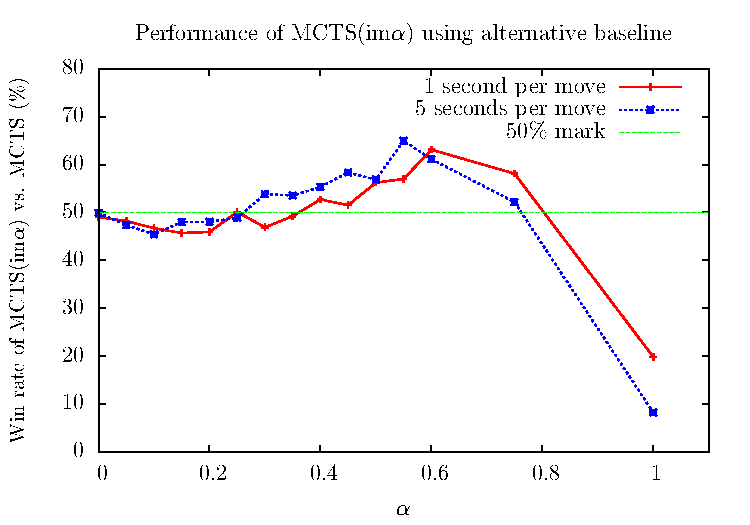
\includegraphics[scale=0.68]{plots/bt-alt-alpha}
\caption{Results of varying $\alpha$ in Breakthrough using the alternative baseline player.
Each point represents 1000 games.} 
\label{fig:bt-alt-alpha}
\end{center}
\end{figure}

\subsubsection*{Comparison to $\alpha\beta$ Search}

% mcts
%                                      ab vs.                   mcts_h_s_ege0.1_det0.5:  1449   551     0 (diff   898, games  2000) 72.45 27.55 +/- 1.96
%                                      ab vs.                   mcts_h_s_ege0.1_det0.5:   610   390     0 (diff   220, games  1000) 61.00 39.00 +/- 3.02
%                                      ab vs.                   mcts_h_s_ege0.1_det0.5:   262   238     0 (diff    24, games   500) 52.40 47.60 +/- 4.38
%
%                                  ab_ev1 vs.              mcts_h_s_ege0.1_det0.5_efv1:  1842   158     0 (diff  1684, games  2000) 92.10 7.90 +/- 1.18
%                                  ab_ev1 vs.              mcts_h_s_ege0.1_det0.5_efv1:   892   108     0 (diff   784, games  1000) 89.20 10.80 +/- 1.92
%                                  ab_ev1 vs.              mcts_h_s_ege0.1_det0.5_efv1:   437    63     0 (diff   374, games   500) 87.40 12.60 +/- 2.91
%                                  ab_ev1 vs.              mcts_h_s_ege0.1_det0.5_efv1:   406    94     0 (diff   312, games   500) 81.20 18.80 +/- 3.42
%                                  ab_ev1 vs.              mcts_h_s_ege0.1_det0.5_efv1:   403    97     0 (diff   306, games   500) 80.60 19.40 +/- 3.47
%                                  ab_ev1 vs.              mcts_h_s_ege0.1_det0.5_efv1:   361   120     0 (diff   241, games   481) 75.05 24.95 +/- 3.87

% im-mcts
%                                      ab vs.             mcts_h_s_ege0.1_det0.5_im0.4:  1099   901     0 (diff   198, games  2000) 54.95 45.05 +/- 2.18
%                                      ab vs.             mcts_h_s_ege0.1_det0.5_im0.4:   384   616     0 (diff  -232, games  1000) 38.40 61.60 +/- 3.01
%                                      ab vs.             mcts_h_s_ege0.1_det0.5_im0.4:   191   309     0 (diff  -118, games   500) 38.20 61.80 +/- 4.26

%                                  ab_ev1 vs.        mcts_h_s_ege0.1_det0.5_im0.4_efv1:  1519   481     0 (diff  1038, games  2000) 75.95 24.05 +/- 1.87
%                                  ab_ev1 vs.        mcts_h_s_ege0.1_det0.5_im0.4_efv1:   727   273     0 (diff   454, games  1000) 72.70 27.30 +/- 2.76
%                                  ab_ev1 vs.        mcts_h_s_ege0.1_det0.5_im0.4_efv1:   337   163     0 (diff   174, games   500) 67.40 32.60 +/- 4.11
%                                  ab_ev1 vs.        mcts_h_s_ege0.1_det0.5_im0.4_efv1:   292   208     0 (diff    84, games   500) 58.40 41.60 +/- 4.32
%                                  ab_ev1 vs.        mcts_h_s_ege0.1_det0.5_im0.4_efv1:   277   223     0 (diff    54, games   500) 55.40 44.60 +/- 4.36
%                                  ab_ev1 vs.        mcts_h_s_ege0.1_det0.5_im0.4_efv1:   237   263     0 (diff   -26, games   500) 47.40 52.60 +/- 4.38


%Through systematic testing, we found the best baseline with this evaluation 
%function to use the pd$20$ playout. 

\begin{table}[t]
{\small
\begin{center}
\begin{tabular}{ccccc|c}
Ev. Func.  & Player              & Opp.                 & $n$    & $t$ (s) & Res. (\%) \\
\hline
(Both)     & $\alpha\beta$(efMS) & $\alpha\beta$(efLH)  & 2000   & 1       & 70.40     \\
(Both)     & $\alpha\beta$(efMS) & $\alpha\beta$(efLH)  &  500   & 5       & 53.40     \\
(Both)     & $\alpha\beta$(efMS) & $\alpha\beta$(efLH)  &  400   & 10      & 31.25     \\
\hline
\hline
efMS       & MCTS              & $\alpha\beta$    & 2000   & 1       & 27.55     \\     
efMS       & MCTS              & $\alpha\beta$    & 1000   & 5       & 39.00     \\     
efMS       & MCTS              & $\alpha\beta$    &  500   & 10      & 47.60     \\     
\hline
efMS       & MCTS(im$0.4$)     & $\alpha\beta$    & 2000   & 1       & 45.05     \\     
efMS       & MCTS(im$0.4$)     & $\alpha\beta$    & 1000   & 5       & 61.60     \\     
efMS       & MCTS(im$0.4$)     & $\alpha\beta$    &  500   & 10      & 61.80     \\     
\hline
\hline
efLH       & MCTS              & $\alpha\beta$    & 2000   & 1       &  7.90      \\     
efLH       & MCTS              & $\alpha\beta$    & 1000   & 5       & 10.80      \\     
efLH       & MCTS              & $\alpha\beta$    &  500   & 10      & 12.60      \\     
efLH       & MCTS              & $\alpha\beta$    &  500   & 20      & 18.80      \\     
efLH       & MCTS              & $\alpha\beta$    &  500   & 30      & 19.40      \\     
efLH       & MCTS              & $\alpha\beta$    &  500   & 60      & 24.95      \\     
efLH       & MCTS              & $\alpha\beta$    &  130   & 120     & 25.38      \\     
\hline
efLH       & MCTS(im$0.6$)     & $\alpha\beta$    & 2000   & 1       & 28.95      \\     
efLH       & MCTS(im$0.6$)     & $\alpha\beta$    & 1000   & 5       & 39.30      \\     
efLH       & MCTS(im$0.6$)     & $\alpha\beta$    &  500   & 10      & 41.20      \\     
efLH       & MCTS(im$0.6$)     & $\alpha\beta$    &  500   & 20      & 45.80      \\     
efLH       & MCTS(im$0.6$)     & $\alpha\beta$    &  500   & 30      & 46.20      \\     
efLH       & MCTS(im$0.6$)     & $\alpha\beta$    &  500   & 60      & 55.60      \\     
efLH       & MCTS(im$0.6$)     & $\alpha\beta$    &  130   & 120     & 61.54      \\     
\hline
\end{tabular}
\end{center}
\caption{Summary of results versus $\alpha\beta$. 
Here, $n$ represents the number of games played and $t$ time in seconds per search.
Win rates are for the Player (in the left column).}
\label{tbl:ab_vs_mcts}
}
\end{table}

Since implicit minimax backups enhances MCTS by using minimax-style updates, a natural 
question is how it compares to $\alpha\beta$ search. 
So, here we compare MCTS with implicit minimax backups versus $\alpha\beta$ search.
Our $\alpha\beta$ search player uses iterative deepening and a static move ordering. 
The static move ordering is based on the same information used in the informed playout
policies: decisive and anti-decisive moves are first, then captures of defenseless pieces, 
then all other captures, and finally regular moves.
The results are listed in Table~\ref{tbl:ab_vs_mcts}.

The first observation from these results is that the performance of MCTS increases versus 
$\alpha\beta$ as search time increases. This is true in all cases, using either evaluation function, 
with and without implicit minimax backups. This is similar to previous observations in 
Lines of Action~\cite{Winands11AB} and multiplayer search~\cite{Sturtevant08icga,Nijssen13}.

The second observation is that in every case, MCTS(im$\alpha$) performs significantly better 
against $\alpha\beta$ than the baseline player at the same search time. 
Using efMS in Breakthrough with 5 seconds of search time, MCTS(im$0.4$) performs significantly 
better than both the baseline MCTS player and $\alpha\beta$ search on their own. 

The third observation is that MCTS(im$\alpha$) benefits quite significantly from weak 
heuristic information, more so than $\alpha\beta$. 
When using efMS, MCTS takes less long to do better against $\alpha\beta$, possibly because MCTS makes 
better use of weaker information. 
When using efLH, $\alpha\beta$ preforms significantly better against MCTS at low time settings.  
However, it is not quite clear whether this due to $\alpha\beta$ improving or MCTS worsening (indeed, 
in the previous subsection we showed that the best implicit minimax player is the one that uses 
the simpler evaluation function.) Therefore, we also include a comparison of the $\alpha\beta$ players
using efMS versus efLH. What we see is that at 1 second, efMS benefits $\alpha\beta$ more, but as time 
increases efLH seems to be preferred. 
Nonetheless, when using efLH, there still seems to be a point where, if given enough search time
the performance of MCTS(im$0.6$) surpasses that of $\alpha\beta$. 

\subsection{Lines of Action}

In subsection~\ref{sec:bt}, we compared the performance of MCTS(im$\alpha$) to a basic $\alpha\beta$
search player. Our main question at this point is how MCTS(im$\alpha$) could perform in a game with 
stronger play due to using proven enhancements in both $\alpha\beta$ and MCTS.
For this analysis, we now consider the well-studied game Lines of Action (LOA). 

LOA is a turn-taking alternating-move game played on an 8-by-8 board that uses checkers board and pieces.
The goal is to connect all your pieces into a single connected group (of any size), 
where the pieces are connected via adjacent and diagonals squares. A piece may move in any direction, but the number of squares 
it may move depends on the total number of pieces in the line, including opponent pieces. A piece may jump over its own
pieces but not opponent pieces. Captures occur by landing on opponent pieces. 

The MCTS player is MC-LOA, whose implementation and enhancements are described in \cite{Winands10MCTS-LOA}. 
MC-LOA is a world-champion engine winning the latest Olympiad. The benchmark $\alpha\beta$ player is MIA, the world-best $\alpha\beta$-player 
upon which MC-LOA is based, winning 4 Olympiads. MC-LOA uses MCTS-Solver, progressive bias, and highly-optimized $\alpha\beta$
playouts. MIA includes the following enhancements: static move ordering, iterative deepening, killer moves, history heuristic, enhanced 
transposition table cutoffs, null-move pruning, multi-cut, realization probability search, quiescence search, and negascout/PVS. 
The evaluation function used is the used in MIA~\cite{Winands06MIA}.
All of the results in LOA are based 100 opening board 
positions.\footnote{\small https://dke.maastrichtuniversity.nl/m.winands/loa/} 

\begin{figure}[t]
\begin{center}
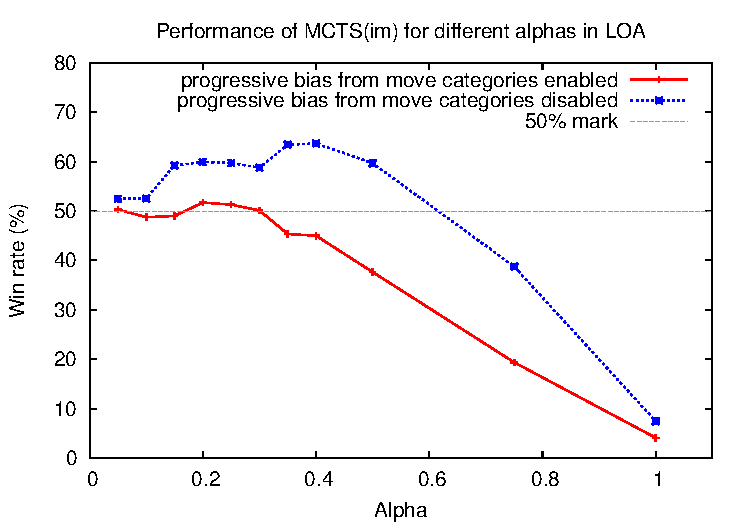
\includegraphics[scale=0.7]{plots/loa-alpha}
\caption{Results in LOA. Each data point represents 1000 games with 1 second of search time. } 
\label{fig:loa-alpha}
\end{center}
\end{figure}

\begin{table}[t]
{\small
\begin{center}
\begin{tabular}{ccccc|c}
Options & Player        & Opp. & $n$ & $t$ & Res. (\%) \\
\hline
\hline
PB      & MCTS(im$\alpha$) & MCTS     & 32000 & 1        & 50.59       \\
PB      & MCTS(im$\alpha$) & MCTS     & 6000  & 5        & 50.91       \\
\hline
$\neg$PB & MCTS(im$\alpha$) & MCTS & 1000 & 1  & 59.90       \\
$\neg$PB & MCTS(im$\alpha$) & MCTS & 6000 & 5  & 63.10       \\
$\neg$PB & MCTS(im$\alpha$) & MCTS & 2600 & 10 & 63.80       \\
\hline
$\neg$PB & MCTS             & $\alpha \beta$ & 2000 & 5  & 40.0       \\
$\neg$PB & MCTS(im$\alpha$) & $\alpha \beta$ & 2000 & 5 & 51.0       \\
\hline
PB       & MCTS             & $\alpha \beta$ & 20000 & 5  & 61.8       \\
PB       & MCTS(im$\alpha$) & $\alpha \beta$ & 20000 & 5  & 63.3       \\
\hline
\end{tabular}
\end{center}
\caption{Summary of results for players and opponent pairings in LOA. 
All MCTS players use $\alpha \beta$ playouts and MCTS(im$\alpha$) players use $\alpha = 0.2$. 
Here, $n$ represents the number of games played and $t$ time in seconds per search.}
\label{tbl:loaresults}
}
\end{table}


We repeat the implicit minimax backups experiment with varying $\alpha$. At first, we use standard UCT without enhancements 
and a simple playout that is selects moves non-uniformly at random based on the move categories, and uses the early cut-off strategy. 
Then, we enable shallow $\alpha \beta$ searches in the playouts described in~\cite{Winands11AB}. 
Finally, we enable the progressive bias based on move categories. The results for these 
three different settings are shown in Figure~\ref{fig:loa-alpha}. As before, we notice that in the first two situations,
implicit minimax backups with $\alpha \in [0.1,0.5]$ can lead to better performance. When the progressive bias based on move 
categories is added, the advantage diminishes. However, we do notice that $\alpha \in [0.05,0.3]$ seems to not significantly 
decrease the performance. 

Additional results are summarized in Table~\ref{tbl:loaresults}. From the graph, we reran $\alpha = 0.2$ with progressive bias for 
32000 games giving a statistically significant (95\% confidence) win rate of 50.59\%. 
We also tried increasing the search time, in both cases (with and without progressive bias), 
and observed a gain in performance at five and ten seconds. 
In the past, the strongest LOA player was MIA which was based on $\alpha \beta$ search. Therefore, we also test our MCTS with 
implicit minimax backups against an $\alpha \beta$ player based on MIA. When progressive bias is disabled, implicit minimax backups
increases the performance by 11 percentage points. There is also a small increase in performance when progressive bias is enabled. 
Also, at $\alpha = 0.2$, it seems that there is no statistically significant case of implicit minimax backups hurting performance. 

%\subsection{Discussion: Traps and Limitations} 
\subsection{Discussion: Limitations} 

%Add for camera-ready.
%The initial motivation for this work was driven by the trap moves which pose problems in 
%MCTS~\cite{Ramanujan11Tradeoffs,Baier13MinimaxHybrids,Gudmindsson13Sufficiency}. We tried to construct an example board in Breakthrough 
%to demonstrate how implicit minimax backups deals with problems with traps. We were unable to do so, and we suspect the following
%reasons. 
%First, in our experience it seems that traps are effectively handled by improving the playout policy. Even without early terminations, 
%simply having decisive and anti-decisive moves and preferring good capture moves seems to be enough to handle traps in Breakthrough.
%Second, even when using random playouts, with sufficiently high simulations in an efficient implementation, shallow traps seem to be
%handled effectively without any additional knowledge. Therefore, we now believe the explanation for the advantage offered by 
%implicit minimax backups is somewhat more subtle than simply detecting and handling traps. 

While we have shown positive results in a number of domains, we recognize that this 
technique is not universally applicable. We believe that implicit minimax backups work because there is short-term tactical 
information which 
is not captured in the long-term playouts, but is captured by the implicit minimax procedure. Additionally, we suspect that 
there must be strategic 
information in the playouts which is not captured in the shallower minimax backups. Thus, success depends on both the domain and 
the evaluation function used. Implicit minimax backups did not improve performance in Chinese Checkers or the card game Hearts, 
but more work needs to be done to understand if we would find success with a better evaluation function.

\section{Conclusion}

We have introduced a new technique called implicit minimax backups for MCTS. 
Unlike previous methods, this techniques stores 
the information from both sources separately, only combining the two sources to guide
selection. This simple technique can lead to stronger play even with
simple evaluation functions, which is often readily available. 
In Breakthrough, our evaluation shows that implicit minimax backups increases 
the strength of MCTS significantly compared to similar techniques for improving MCTS
using domain knowledge.
Furthermore, the technique improves 
performance in LOA, a larger, more complex domain with sophisticated knowledge and 
strong MCTS and $\alpha \beta$ players. 

In most cases, $\alpha \in [0.15,0.4]$ seems to be a safe range, and we found generally 
that the more knowledge that is already included in the MCTS baseline player, the lower
the optimal $\alpha$ tends to be. In Breakthrough, this range is higher $[0.5,0.6]$ 
when using node priors at lower time settings and when using the alternative baseline. 

For future work, we would like to apply the technique in other games, Amazons in 
particular. 
We hope to compare implicit minimax backups with sufficiency thresholds 
of Gudmundsson \& Bj\"{o}rnsson~\cite{Gudmindsson13Sufficiency} and to other 
minimax hybrids, such as those of Baier \& Winands~\cite{Baier13MinimaxHybrids}. 
%We also plan to investigate decaying strategies for 
%$\alpha$ and incremental $\alpha \beta$ pruning.
The technique could also work in general game-playing agents using 
evaluations learned during search~\cite{Finnsson10Learning}.

\noindent {\bf Acknowledgments.} This work is partially funded by the Netherlands 
Organisation for Scientific Research (NWO) in the framework of the project Go4Nature, grant number 612.000.938. 

\bibliographystyle{IEEEtran}
% argument is your BibTeX string definitions and bibliography database(s)
%\bibliography{IEEEabrv,../bib/paper}
\bibliography{im-mcts}
%
% <OR> manually copy in the resultant .bbl file
% set second argument of \begin to the number of references
% (used to reserve space for the reference number labels box)
%\begin{thebibliography}{1}
%\bibitem{IEEEhowto:kopka}
%H.~Kopka and P.~W. Daly, \emph{A Guide to \LaTeX}, 3rd~ed.\hskip 1em plus
%  0.5em minus 0.4em\relax Harlow, England: Addison-Wesley, 1999.
%\end{thebibliography}


% that's all folks
\end{document}


